\documentclass[DIV10]{scrartcl}

\usepackage[utf8]{inputenc}
\usepackage{url}
\usepackage{hyperref}
\usepackage{graphicx}
\usepackage{enumerate}
  
\makeatletter
\newcommand*{\tol}[1]{$\overline{\hbox{#1}}\m@th$}
\makeatother

\renewcommand{\arraystretch}{1.2}

\author{jmA500 <jm@metweb.de>}
\date{\today}
\title{Keyboard tap to configure an Amiga 500}

\begin{document}
\maketitle
\section{Description}
This little piece of hardware is used to provide some means for
configuring an Amiga 500 with the keyboard. This is to replace at
least some of the small switches that are commonly used to configure
the extensions in an Amiga. The circuit listens to the keys pressed
on the Amiga keyboard and then adjusts some of its output pins. These
pins connect to jumper headers on the extension boards and hence provide some
means to configure these extensions without opening the case or
drilling holes into it.
\begin{center}
  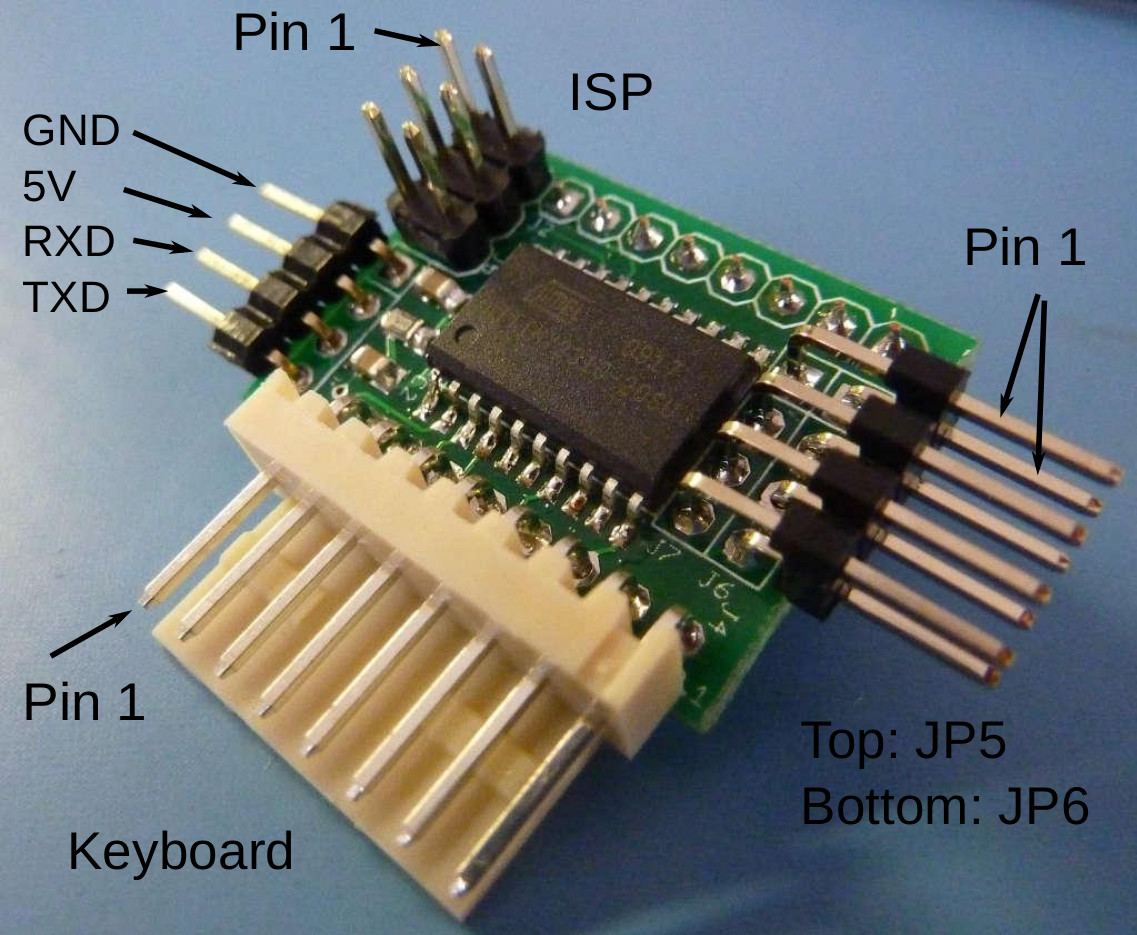
\includegraphics[width=.7\linewidth]{config-annot}
\end{center}
Note however, that this project is not for beginners. If you have
other extensions than I have, you will likely have to adapt the
firmware to your needs. Also, you have to figure out whether your
extensions are configurable by means of an external MCU, that is if is
suffices to drive a signal statically high or low. Switching a dynamic
signal is not possible (without extra hardware)\footnote{I have seen
  some kickstart switches that use a switch to route a signal to
  either of the two ROMs.} 

In any case you need a possibility to program the AtTiny4313
micro-controller with an in system programmer (ISP). These are cheaply
available and connect to USB or parallel port. A lot of information
regarding this micro-controller can be obtained on the
excellent websites \url{http://www.avrfreaks.net/} or
\url{http://www.mikrocontroller.net/} (German).

In addition, if you are not running a Linux machine similar to mine
there might be some extra difficulties adapting the code to your build
environment. In particular I am not using AVR studio and this
distribution does not include any project file for it. However,
pre-built firmware images are included, if you are happy with the
firmware out of the box.

\section{Disclaimer}
I am not responsible for any damages done by this device, and I do not
guarantee that it will work at all. Only connect this to your precious
Amiga, if you are sure about what it does, how it works, and whether
the firmware is what I claim it to be.

\section{Acknowledgments}
The idea to this project was born during a discussion in the
\url{a1k.org/forum} and was suggested by Paradroid. However, if I did
not have all the great hardware extensions created by the community
I would not have had any reason to start the project. Thanks also to
the members of the a1k.org forum encouraging me to continue this project.

\section{License}
All parts of this project are free to use in non-commercial
projects. The firmware is licensed under terms of the GPL 2. Please
quote this document in any derived work. See the file COPYRIGHT in
\verb#src/attiny4313# for additional information, in particular the
reference to Peter Fleury who provided a neat UART library for the
Atmel MCUs.

\section{Hardware}
The hardware is plain and simple, an AtTiny4313 (or 2313) in
minimal configuration with a few pin headers to connect the
configuration jumpers and an ISP Programmer.
In addition, the RxD and TxD pins are accessible on additional
pins.
\begin{center}
  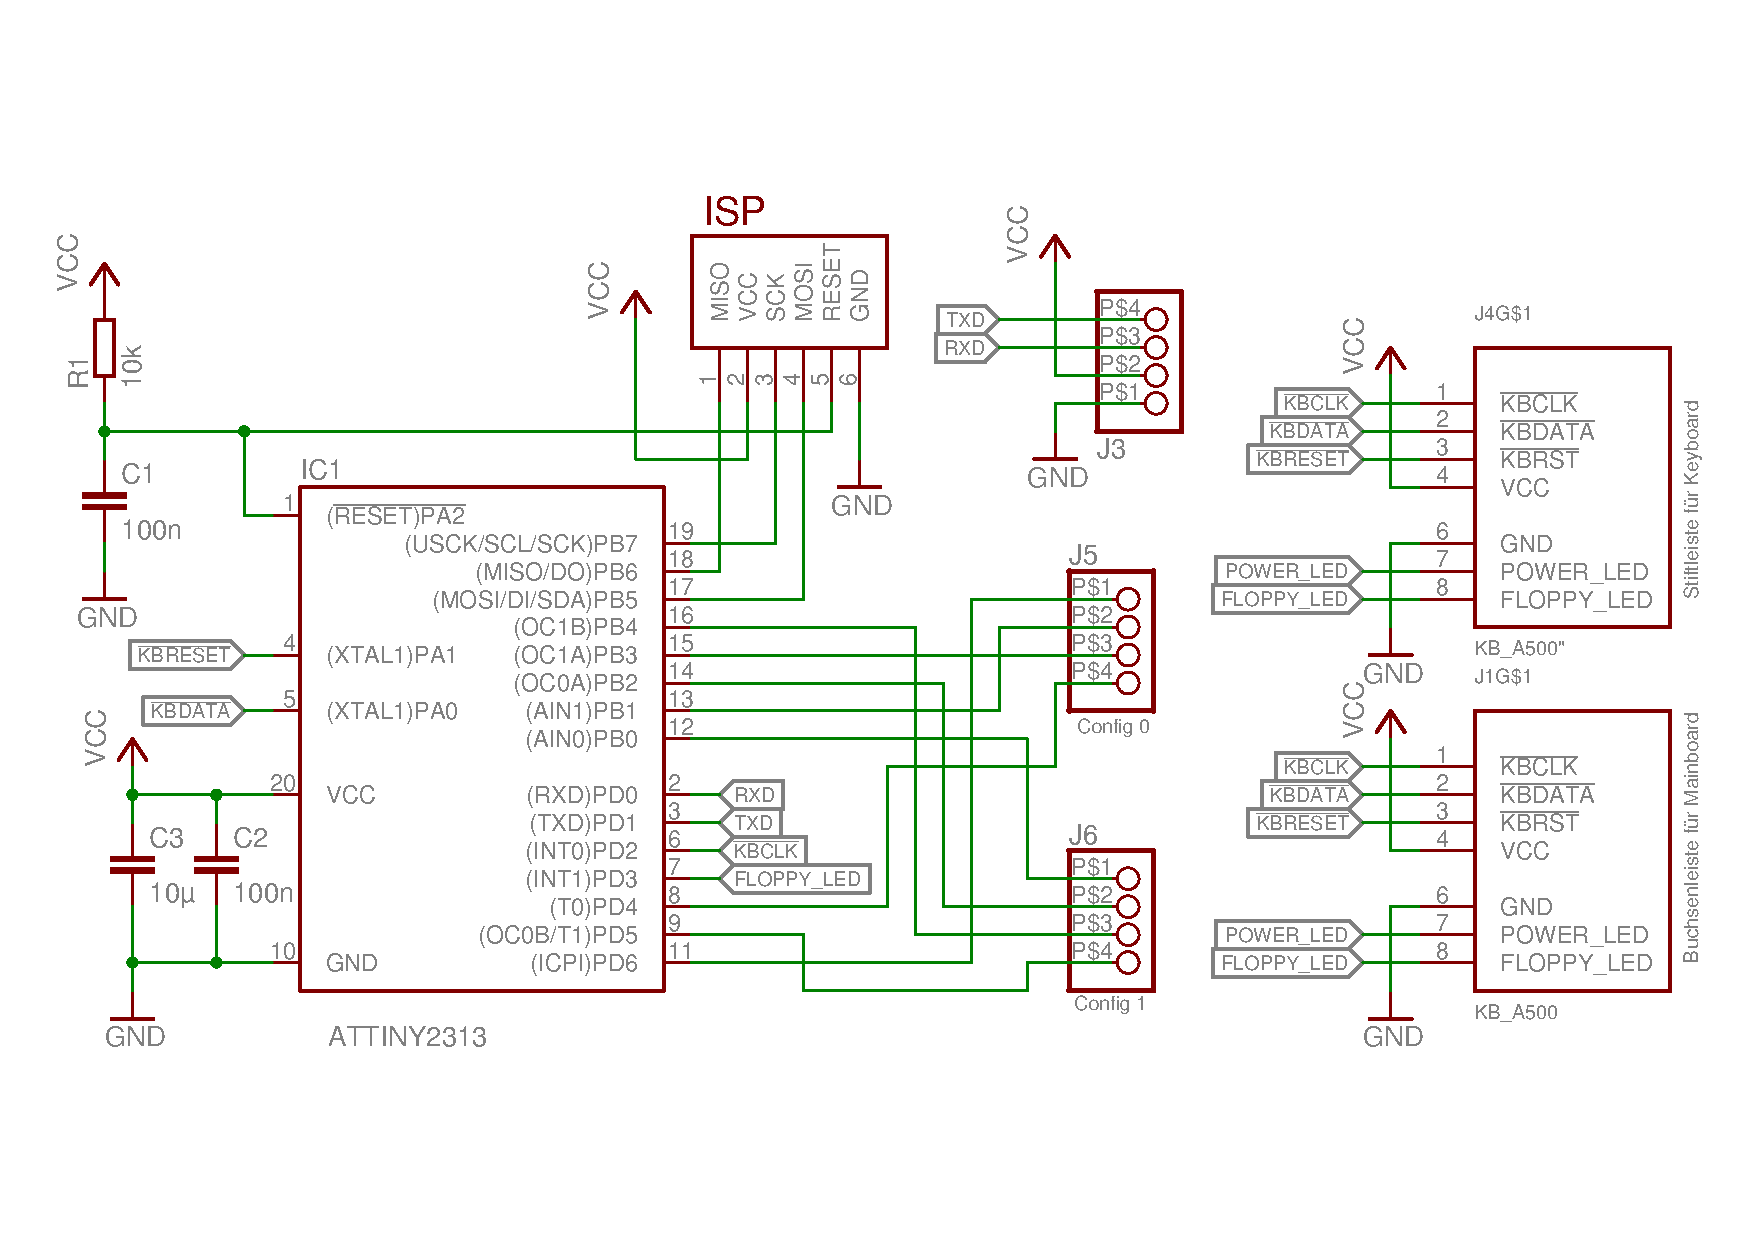
\includegraphics[width=.7\linewidth]{../hardware/schematic.pdf}
\end{center}
There is a board layout done in such a way that the little PCB can be
directly fitted on the keyboard connector on the mainboard of an Amiga
500(+).

However, the whole circuit is so simple that you might consider
building it without a PCB, or you might use an Ardiuno or something
similar. 

\subsection{Part list}
\begin{center}
  \begin{tabular}{|l|l|l|}
    \hline
    IC1 & AtTiny 4313 SO or AtTiny 2313 SO\\
    \hline
    C1,C2 & 100n SMD 0805 \\
    C3 & 10$\mu$ SMD 1206 \\
    R1 & 10k SMD 0805 \\
    \hline
    J1  & 1x8 socket strip 180$^\circ$ 2.54\\
    J2  & 2x3 pinheader 180$^\circ$ 2.54\\
    J3  & 1x4 pinheader 180$^\circ$ 2.54\\
    J4  & 1x8 pinheader 90$^\circ$ 2.54\\
    J5,J6  & 2x4 pinheader 90$^\circ$ 2.54\\
    \hline
  \end{tabular}
\end{center}
For future extensions I suggest using a 4313 with 4k flash and 256
bytes of RAM if you can get one. The firmware distributed along with
this file does not fit the 2313 if the UART functions are enabled. On the other
hand, you may or may not find them useful. Note that I did not
test the board with a 2313{\bfseries A} although that might work
without changing the code.

\subsection{Pin Configuration}
\subsubsection{J1: Connects to A500 mainboard}
\begin{center}
  \begin{tabular}{|l|l|}
  \hline
    1 & \tol{KBCLK} \\
    2 & \tol{KBDATA} \\
    3 & \tol{KBRESET} \\
    4 & VCC \\
    5 & \\
    6 & GND \\
    7 & POWER\_LED \\
    8 & FLOPPY\_LED \\
    \hline
  \end{tabular}
\end{center}
\subsubsection{J2: ISP}
This is to connect an ISP programmer. The pin-out corresponds to Atmel 6-pin
ISP connector. {\bfseries Please make sure that the programmer does not power the
MCU when connected to the A500 mainboard.}
\begin{center}
  \begin{tabular}{|l|l|}
    \hline
    1 & MISO\\
    2 & VCC\\
    3 & SCK\\
    4 & MOSI\\
    5 & \tol{RESET}\\
    6 & GND\\ \hline
  \end{tabular}
\end{center}

\subsubsection{J3: Serial connector}
This is a serial connection with 5V logic levels. Names are from the
perspective of the MCU, so you have to connect the TxD of your
computer to the RxD on the PCB.
\begin{center}
  \begin{tabular}{|l|l|}
    \hline
    1 & GND \\
    2 & VCC \\
    3 & RxD \\
    4 & TxD \\ \hline
  \end{tabular}
\end{center}
The firmware will output some status messages here, and listens to
commands via a small parser. Have a look at the software how to use
it (or send the string \verb#help# to see a small help message). 

\subsubsection{J4:  Connect your keyboard here}
Same as J1.

\subsection{J5, J6: Connectors for configuration jumpers}
\label{sec:config-jumpers}
These connectors provide 8 pins to configure the hardware. Everything
that happens on these pins depends on the firmware. The software
provided with this documentation emulates open collector outputs, ie.\
it will either pull pins low or let them float (configure as inputs)
but never pull them high.

This version of the firmware is used to configure generic devices. The
PCB provides eight independent outputs that can be connected to
various jumpers. You can configure my 1.8/2MB Ranger memory
extension \cite{Memory}, a Kickflash \cite{Kickflash-Thread,Kickflash-Manual} and
the 68010@14MHz Turbo card by Matze \cite{Turbokarte} or any other
device that has jumpers that can be activated by pulling them
low. This includes any standard 512k memory extension.  The Pins are
labeled as follows:
\begin{center}
  \begin{tabular}{|ll|l|}
    \hline
    J5 & 1 & C1 \\
    & 2 & C2 \\
    & 3 & C2 \\
    & 4 & C4 \\
    \hline
    J6 & 1 & C5 \\
    & 2 & C6 \\
    & 3 & C7 \\
    & 4 & C8
    \\ \hline
  \end{tabular}
\end{center}
\begin{enumerate}[Note 1:]
\item \label{item:remark-memory} If you want to control a standard
  512k expansion, connect one of the config pins instead of the
  switch. The switch connector on such a memory expansion has one pin
  which is connedted to ground, the other one is pulled high. Connect
  to the pin which is pulled high.
\end{enumerate}

\section{Firmware}
The firmware for the Atmel is written in C and compiles with avr-gcc
4.8.2 but may or may not compile with different versions although I
tried to be as compatible as possible. The directory \verb#firmware#
contains precompiled flash and eeprom images in Hex-format for the
AtTiny 2313 and 4313. For both MCUs the fuses setting is
\begin{quote}
  \verb#LFUSE = 0xD4, HFUSE = 0xDB, EFUSE = 0xFF#.
\end{quote}
Make sure to program both the flash memory with the corresponding
\verb#.hex# file and the eeprom memory with the \verb#.eep#
file. Never attempt to flash the MCU while plugged into a running
Amiga 500, since it will switch configuration when finished
programming. This could damage your Amiga.

The Makefile provided in the \texttt{src} directory should do the job
by simply running \texttt{make}. If compiling for an AtTiny2313 you
must adjust the \texttt{MCU} variable in the Makefile to read
\texttt{MCU = attiny2313}. Also flash is too tight to use UART
debugging. To disable it, open \verb#main.c# and comment out the line
\verb!#define UART_DEBUG 1!. If you want to use the UART features, us
an AtTiny4313. If you happen to have a USBasp ISP programmer
\cite{USBasp} you can program the MCU by simply running \texttt{make
  fuses} and \texttt{make program}. The Makefile supports programming
with avrdude, the programmer is selected with the variable
\verb#AVRDUDE_PROG#.

The source code should be mostly self explanatory\footnote{An
  obviously biased judgment YMMV.}, although small code
has been preferred to readable code in some places. The crucial global
variable is \verb#conf#. There are two bytes, \verb#current# and
\verb#next#. Each bit in those variables corresponds to one config
pin.  {\bfseries A one in these bits
  results in pulling the corresponding pin low.}
The main loop checks whether one of the F-keys is pressed before the
\emph{Help}-key gets pressed three times and changed the next
configuration accordingly. If it detects a keyboard reset the new
configuration gets written to the pins and is stored in the eeprom. 

\section{Usage}
This is the selections available if the configurator is connected as
described in section~\ref{sec:config-jumpers} and programmed with the
\emph{generic} firmware. The keys F1-F8 are used to switch the
configuration pins as follows:
\begin{center}
  \begin{tabular}{|l|l||l|l|}
    \hline
    F1 & set C1 & Shift+F1 & clear C1 \\
    F2 & set C2 & Shift+F2 & clear C2 \\
    F3 & set C3 & Shift+F3 & clear C3 \\
    F4 & set C4 & Shift+F4 & clear C4 \\
    F5 & set C5 & Shift+F5 & clear C5 \\
    F6 & set C6 & Shift+F6 & clear C6 \\
    F7 & set C7 & Shift+F7 & clear C7 \\
    F8 & set C8 & Shift+F8 & clear C8 \\
    \hline
  \end{tabular}
\end{center}
To change the configuration proceed as follows:
\begin{enumerate}
\item Push \emph{Fx} or \emph{Shift-Fx} if you intend to enable (resp. disable)
  configuration pin \emph{x}.
\item Hit the \emph{Help}-key three times. This changes the next
  configuration that gets activated but does not yet switch the
  configuration pins.
\item You can repeat steps 1 and 2 to change further pins.
\item To activate the configuration perform a keyboard reset. This
  also stores the new configuration setting to eeprom so that it loads
  on the next power on.
\end{enumerate}
  
If you accidentally select a configuration that does not run and is
screwed in such a way that the keyboard is not initialized, you can do
a keyboard reset for at least 6 seconds to load the hopefully save
configuration where all pins are disabled. This fail-safe
configuration is defined by the macro \verb!CONFIG\_DEFAULT! in the
file \verb#ee\_helper.h#.

\bibliographystyle{plain}
\bibliography{references}

\end{document}

%%% Local Variables: 
%%% mode: latex
%%% TeX-master: t
%%% End: 
